\documentclass{article}
\usepackage[utf8]{inputenc}
\usepackage{graphicx}
\graphicspath{ {./} 

\title{Analytical Solution of Poisson-Boltzmann Equation for a Point Charge Surrounded by Ions}
\author{Georgy Derevyanko & Talant Ruzmetov }
\date{October 2019}

\begin{document}

\maketitle

\section{Problem Setup}

Generalized non-linear PB equation with in-homogeneous dielectric constant has the following form:
\begin{equation}
  \label{eq:GPB}
  \nabla \cdot \left( \varepsilon(\mathbf{r}) \nabla \phi(\mathbf{r}) \right) +
  k_{0}^2 \lambda(\mathbf{r}) \phi(\mathbf{r}) = -\frac{4\pi \rho}{\epsilon_0}.   
\end{equation}

Formulation:
A single atom with charge $q$ located at position $\mathbf{r}_0$ in a solvent with density $\rho_0$, and
surrounded with positive ($e^{+}$) and negatively charged ($e^{-}$) ions with bulk concentration $n_0$:
The non-linear part of the PB equation is simplified assuming ion density around an atom(or molecule) obey
Boltzmann distribution:


\begin{equation}
  \label{eq:BoltzDist}
    n_{i} = \lambda(\mathbf{r}) n_0 \exp \left(\frac{ q_i \phi(\mathbf{r})}{k_B T} \right) 
\end{equation}
, where $\lambda$ is a masking function introduced to model Stern layer, which is a region around the solute
from which ions are excluded:
\begin{equation}
  \label{eq:MaskF}
    \lambda(r) = 1 - \exp\left( \frac{-(\mathbf{r}-\mathbf{r}_0)^2}{(\sigma+\sigma_{S})^2} \right).
\end{equation}

The dielectric constant is smoothly distributed throughout the volume using Gaussian function.
\begin{equation}
  \label{eq:GaussEps}
    \varepsilon(\mathbf{r}) = \varepsilon_{out} + (\varepsilon_{in} - \varepsilon_{out})\exp\left( \frac{-(\mathbf{r}-\mathbf{r}_0)^2}{\sigma^2} \right),
\end{equation}


%
\begin{figure}
  \begin{centering}
    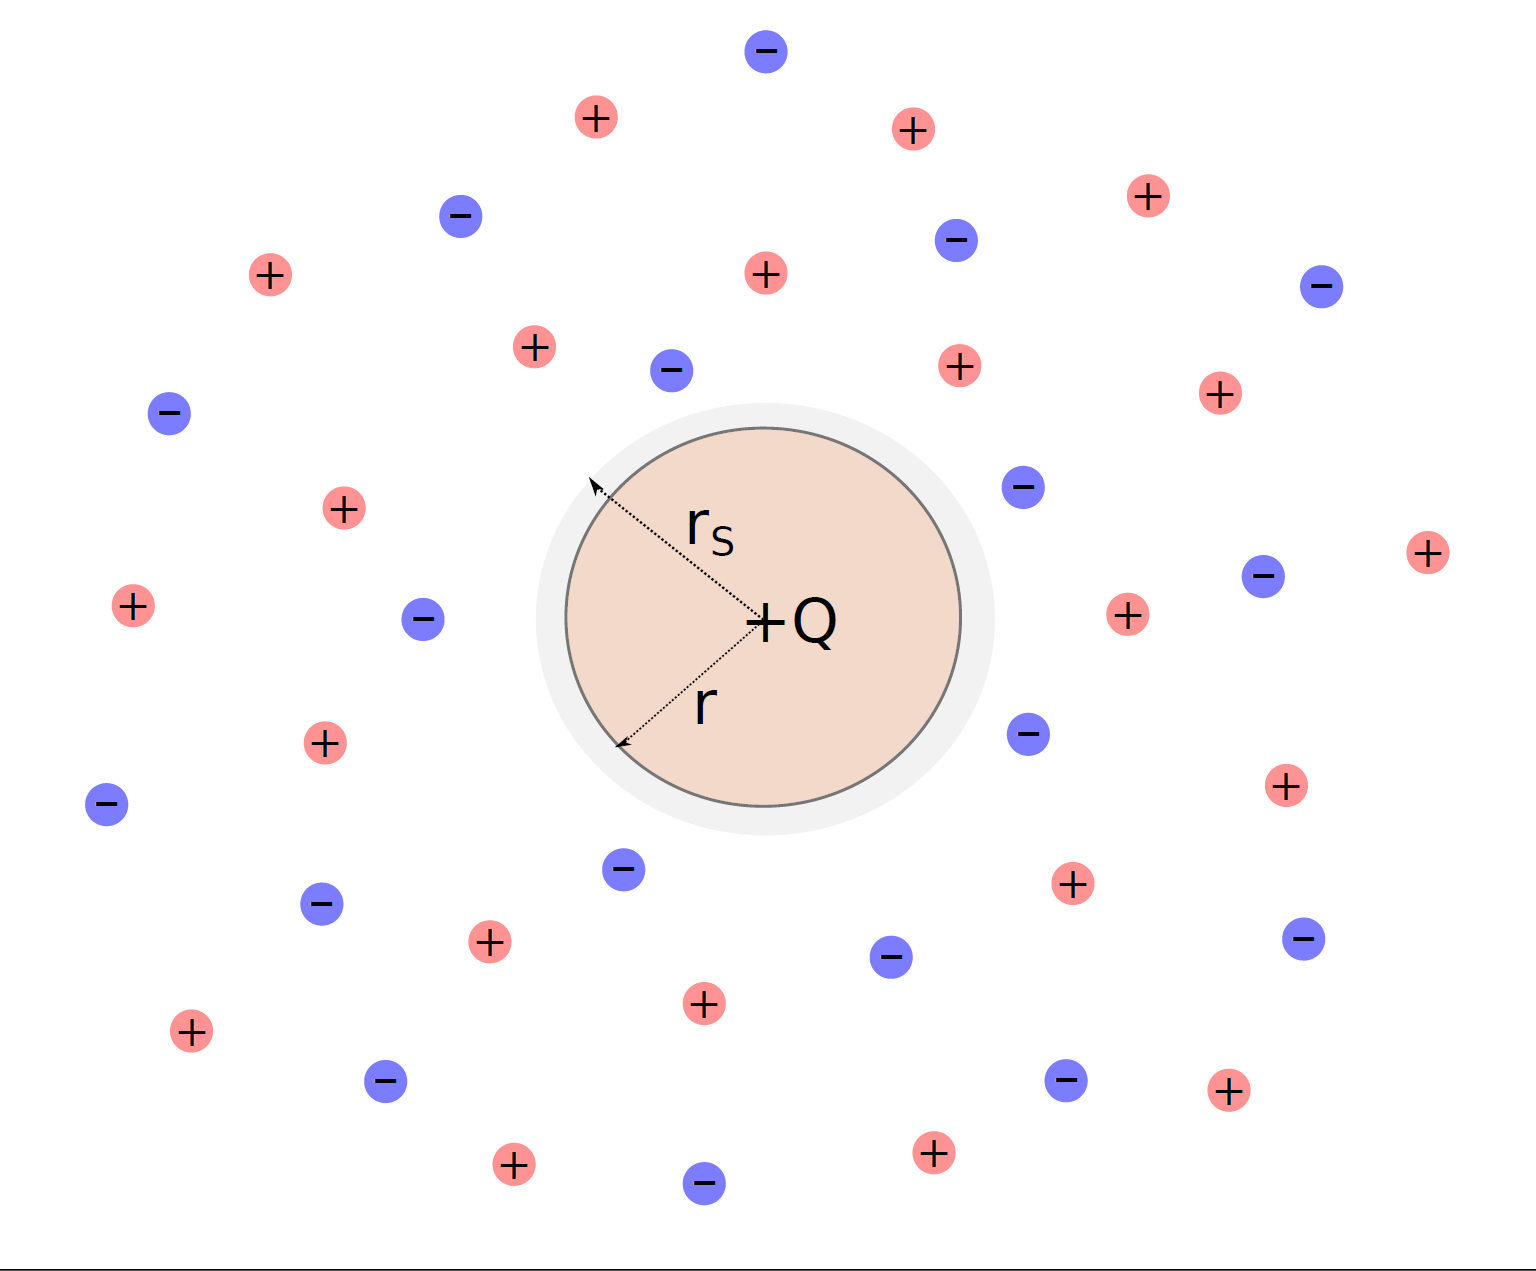
\includegraphics[width=8.0cm]{Figure1.png}
    \caption{ }
    \label{fig:phi_r}
  \end{centering}
\end{figure}
%

In this, $\varepsilon_{out}$ is dielectric constant of the solvent(usually water 79.0), and
$\varepsilon_{in}$ is a reference minimum dielectric constant that represents compact solvent void regions, 
such as hydrophobic core of the folded protein. $\sigma$ is a size of an atom. \newline

Charge:
\begin{equation}
  \label{eq:Charge}
    \rho(\mathbf{r}) = q\delta(\mathbf{r} - \mathbf{r}_0)
\end{equation}

Parameter $k_0$

\begin{equation}
  \label{eq:k0}
    k_{0} = \frac{2 N_{A} e^2 \rho_{0} I}{k_B T} 
\end{equation}

Ionic strength is estimated assuming ions carry either $+e$ or $-e$ charges, also
number of positive and negative ions are same $n_{+} = n_{-} = n_0$.
\begin{equation}
  \label{eq:IonStrength}
    I = \frac{n_0}{N_A \rho_0}.
\end{equation}
Here, $\rho_0$ is solvent density, that is usually water.

\textbf{Task}: Solve for $\phi(\mathbf{r})$

\section{Solution}

First, let's simplify Equ.~\ref{eq:GPB}. The first term can be simplified in the following way:
\begin{equation}
    \label{eq:PBTerm1}
        \nabla \cdot \left( \varepsilon(\mathbf{r}) \nabla \phi(\mathbf{r}) \right) = 
        \nabla \cdot \left( \varepsilon(\mathbf{r}) \frac{\partial \phi}{\partial x}   \hat{x} +
        \varepsilon(\mathbf{r}) \frac{\partial\phi}{\partial y} \hat{y} +
        \varepsilon(\mathbf{r}) \frac{\partial \phi}{\partial z} \hat{z}) \right) = 
        %\frac{\varepsilon(\mathbf{r})}{dx} \frac{d\phi}{dx} +
        %\frac{\varepsilon(\mathbf{r})}{dy} \frac{d\phi}{dy} + 
        %\frac{\varepsilon(\mathbf{r})}{dz} \frac{d\phi}{dz} +
        %\varepsilon(\mathbf{r}) \nabla^2 \phi(\mathbf{r}) =  
        \nabla \varepsilon(\mathbf{r}) \cdot \nabla \phi(\mathbf{r}) +
        \varepsilon(\mathbf{r}) \nabla^2 \phi(\mathbf{r})
\end{equation}
Now, we make coordinate transformation to spherical coordinate system, where derivatives
are taken with respect to $r$, $\theta$, $\psi$.
\begin{equation}
  \label{eq:DelEps}
    \nabla \varepsilon = \frac{\partial \varepsilon}{\partial r} \hat{r} +
    \frac{1}{r} \frac{\partial \varepsilon}{\partial \theta} \hat{\theta} +
    \frac{1}{r \sin{\theta}} \frac{\partial \varepsilon}{\partial \psi} \hat{\psi} \\
\end{equation}

\begin{equation}
  \label{eq:DelPhi}
    \nabla \phi = \frac{\partial \phi}{\partial r} \hat{r} +
    \frac{1}{r} \frac{\partial \phi}{\partial \theta} \hat{\theta} +
    \frac{1}{r \sin{\theta}} \frac{\partial \phi}{\partial \psi} \hat{\psi} 
\end{equation}


\begin{equation}
  \label{eq:DelPhiDotDelEps}
    \nabla \varepsilon \cdot \nabla \phi  = \frac{\partial \varepsilon}{\partial r}
    \frac{\partial \phi}{\partial r} +
    \frac{1}{r^2} \frac{\partial \varepsilon}{\partial \theta}
    \frac{\partial \phi}{\partial \theta} +
    \frac{1}{r^2 \sin{\theta}^2} \frac{\partial \varepsilon}{\partial \psi} 
    \frac{\partial \phi}{\partial \psi} +
\end{equation}

\begin{equation}
  \label{eq:EpsNableSquarePhi}
    \varepsilon \nabla^2 \phi  = \frac{\varepsilon}{r^2} \frac{\partial }{\partial r}
    \left( r^2 \frac{\partial \phi}{\partial r} \right) +
    \frac{\varepsilon}{r^2 \sin{\theta}} \frac{\partial}{\partial \theta}
    \left( \sin{\theta} \frac{\partial \phi}{\partial \theta} \right) +
    \frac{\varepsilon}{r^2 \sin{\theta}^2} 
    \frac{\partial^2 \phi}{\partial \psi^2}
\end{equation}

Normally, separation of variables is performed in order to separate radial and angular parts of
equation. Here, since we have only 1 charged atom, we can assume spherical symmetry and drop all
angular derivatives. Then, Equ.~\ref{eq:GPB} simplifies to the following:

\begin{equation}
    \label{eq:PB1}
        \frac{\partial \varepsilon}{\partial r} \frac{\partial \phi}{\partial r} +
        \frac{\varepsilon}{r^2} \frac{\partial}{\partial r}
        \left( r^2 \frac{\partial \phi}{\partial r}\right)
        + k_{0}^{2} \lambda(r) \phi = -\frac{4\pi \rho(r)}{\epsilon_0}
\end{equation}

Let's expand the second term and plug the expression for $\lambda$. Also, for simplicity
let's put the atom at origin. Then,  $r_0=0$,  $(\mathbf{r} - \mathbf{r}_0)^2 = r^2 $.

\begin{equation}
    \label{eq:PB2}
        \frac{\partial \varepsilon}{\partial r} \frac{\partial \phi}{\partial r} +
        \varepsilon \frac{\partial^2 \phi}{\partial r^2} +
        \frac{2\varepsilon}{r} \frac{\partial \phi}{\partial r} +
        k_{0}^{2} \left( 1 - \exp \left(- \frac{r^2 }{\sigma + \sigma_S} \right) \right) \phi = -\frac{4\pi \rho(r)}{\epsilon_0}
\end{equation}
Including derivatives of $\varepsilon$ into the equation we can arrive at finale second order differential equation:

\begin{equation}
    \label{eq:PB3}
    %\left( \varepsilon_{out} + \exp\left(-\frac{r^2}{\sigma^2}\right) (\varepsilon_{in} - %\varepsilon_{out}) \right)
    \varepsilon(r) \phi'' + \frac{2}{r \sigma^2}(r^2 \varepsilon_{out} - r^2 \varepsilon(r) +
    \sigma^2 \varepsilon(r)) \phi' + k_0^2 \left(  1 - \exp \left(- \frac{r^2 }{\sigma + \sigma_S} \right)  \right) \phi = 
    -\frac{4\pi q \delta(r)}{\epsilon_0}
\end{equation}

So, based on this complicated form, it is probably gonna be hard to make a good guess for 
the form of solution. The numerical solution with \textit{python}  might be more feasible.

Final Equ:
\begin{equation}
    \label{eq:PB4}
    \varepsilon(r) \phi'' + (\varepsilon'(r) + \frac{2}{r} \varepsilon) \phi'
    + k_0^2 \lambda(r) \phi = -\frac{4\pi q \delta(r)}{\epsilon_0}
\end{equation}

%
\begin{figure}
  \begin{centering}
    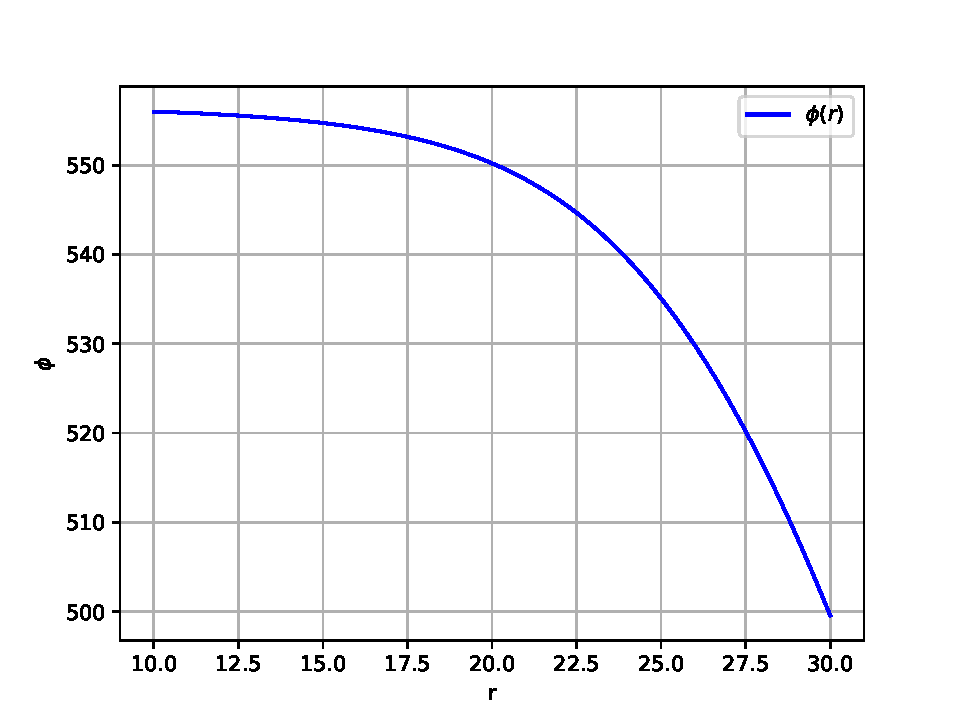
\includegraphics[width=12.0cm]{Figure2.pdf}
    \caption{Electrostatic potential vs radial distance is plotted for spherical charge distribution.
      Value of the potential at the surface of sphere is feeded to code as initial value of potential
      because it can be easyli estimated. Assuming charges are uniformly distributed over the surface of sphere
      one can find a potential inside or at the surface of the sphere from following ralation:
      $\phi = \frac{1}{4 \pi \varepsilon_0} q/\sigma$. }
    \label{fig:phi_r}
  \end{centering}
\end{figure}
%


\end{document}
